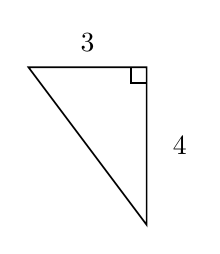
\begin{tikzpicture}[x=1cm,y=1cm,font=\normalsize,
 geometry edge/.style={solid,line width=.6pt},
 geometry mark/.style={solid,line width=.6pt},
 geometry label/.style={font=\normalsize,inner sep=2pt}]
\coordinate (T) at (0,0);
\coordinate (R) at (1.5,0);
\coordinate (B) at (1.5,-2);
\draw[geometry edge] (T)--(R)--(B)--cycle;
\draw[geometry mark] (1.3,0)--(1.3,-0.2)--(1.5,-0.2);
\node[font=\normalsize,inner sep=2pt,fill=white] at (0.75,0.32) {$3$};
\node[font=\normalsize,inner sep=2pt,fill=white] at (1.92,-1) {$4$};
\end{tikzpicture}
